\begin{circuitikz}[background rectangle/.style={fill=white}, show background rectangle]
        \node(0,0) {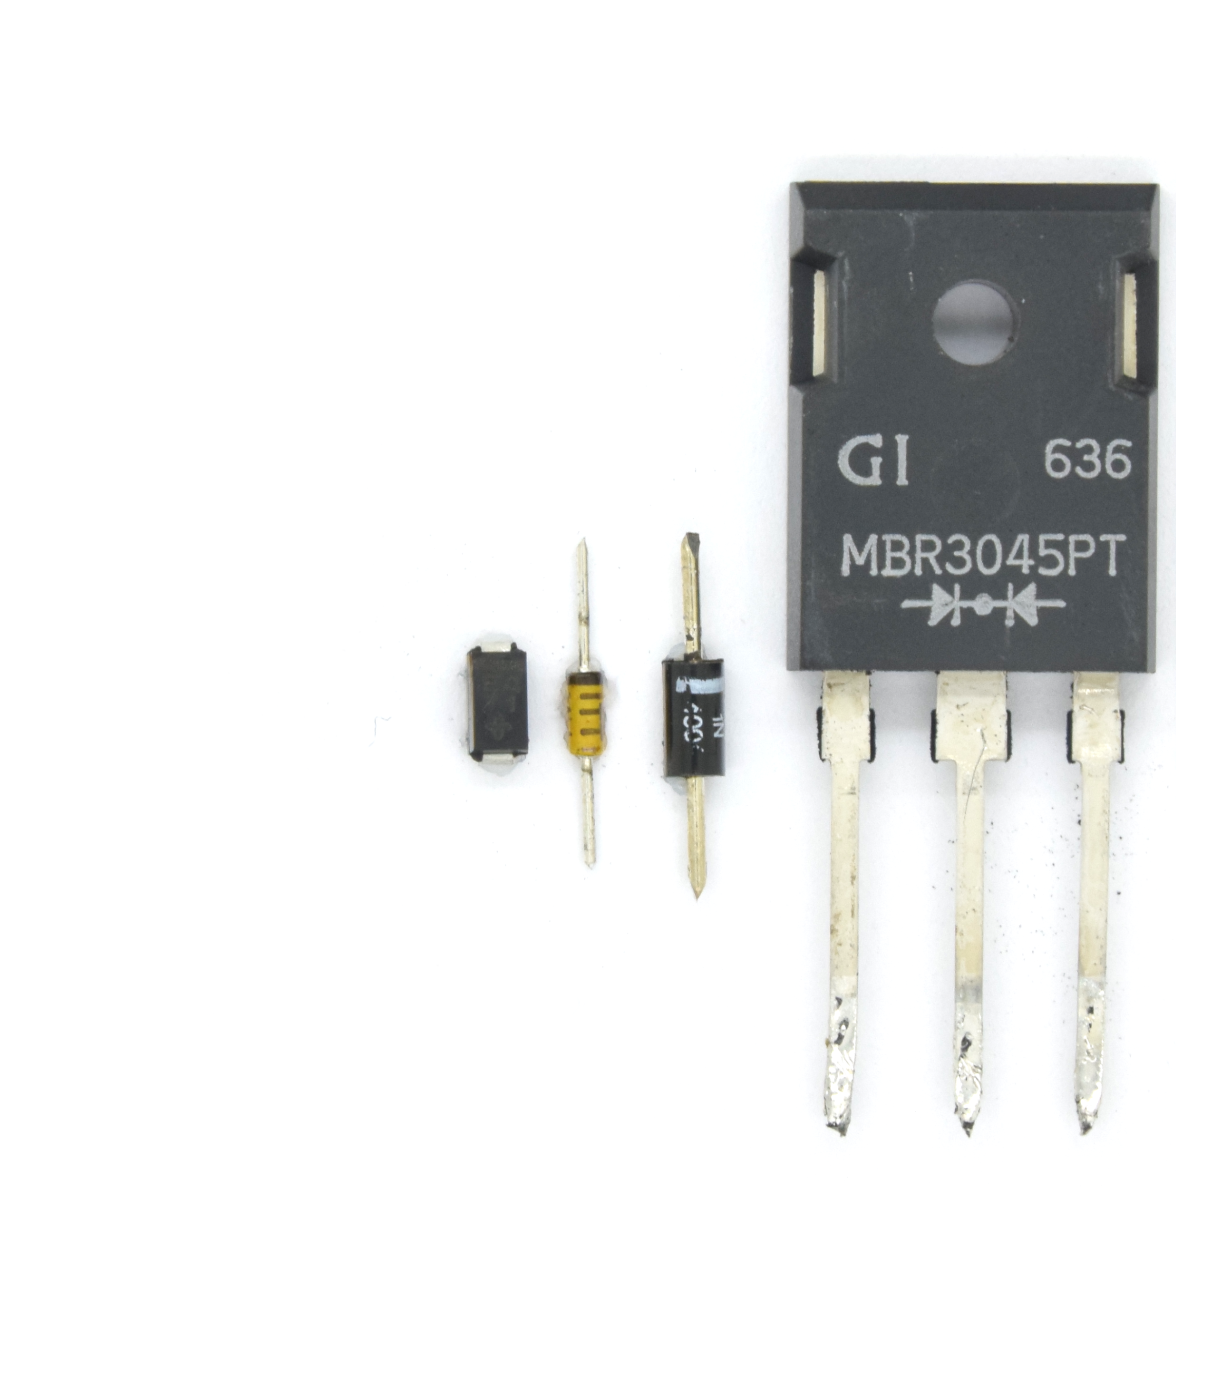
\includegraphics[width=200pt]{foto/7}};
        
        \draw(-3.0,1) to [stroke diode, invert, european,l={$D$}] ++(0,-2);
    
        % Beschriftung:
        \draw( 2.00,  3.50) node {\small MBR3045PT};
        \draw( 2.00, -3.00) node {\small \qty{45}{\volt} / \qty{30}{\ampere}};
        \draw( 0.50,  1.75) node[rotate=90] {\small 1N4007};
        \draw( 0.50, -2.35) node[rotate=90] {\small \qty{1000}{\volt} / \qty{1}{\ampere}};
        \draw(-0.10,  1.75) node[rotate=90] {\small 1N4148};
        \draw(-0.10, -2.35) node[rotate=90] {\small \qty{100}{\volt} / \qty{200}{\milli\ampere}};
        \draw(-0.65,  1.10) node[rotate=90] {\small EGF1A};
        \draw(-0.65, -1.45) node[rotate=90] {\small \qty{50}{\volt} / \qty{1}{\ampere}};
    
        % Pfeile:
        \draw[>=triangle 60, <->] (-1.6,0.675) coordinate(c1) -- ++(0,-1.35) coordinate(c2);
        \draw(c1) -- ++( 0.25,0);
        \draw(c1) -- ++(-0.25,0);
        \draw(c2) -- ++( 0.25,0);
        \draw(c2) -- ++(-0.25,0);
    
        % Text:
        \draw (c1) ++ (0,0.25) node {\qty{1}{\centi\meter}};
    
\end{circuitikz}